% Appendix

\section{Dataset and Split Details}
\label{app:data}

\subsection{ScienceWorld Task Types}

Table~\ref{tab:sw_tasks} lists the ScienceWorld task types used for training and out-of-distribution evaluation.

\input{tables/sw_tasks}

For each task type, we sample up to 30 variations (to bound collection time). Variations are split 60\%/20\%/20\% into train/validation/test using a fixed random seed (42).

\subsection{HLE Subject Categories}

\input{tables/hle_categories}

\section{Error Detection Rules}
\label{app:error_rules}

Table~\ref{tab:error_rules_detail} provides the full specification of error detection rules used to compute annealed error costs (AEC) during training.
Each rule consists of pattern strings matched against environment observations, a severity level (high/medium/low), and a description.

\paragraph{Design Principles.}
For HLE, we distinguish between model errors (format violations, Python exceptions) and external failures (HTTP errors, paywalls).
Model errors receive higher severity since they reflect controllable mistakes; external failures are marked low severity as they depend on third-party services.
For ScienceWorld, we only penalize truly invalid actions (commands not recognized by the environment parser).
Environmental feedback such as ``the door is not open'' or ``the object is already in your inventory'' represents normal exploration and is not treated as an error.

\paragraph{Severity Coefficients.}
Severity levels map to penalty coefficients in AEC: high (1.0), medium (0.8), low (0.2).
The warmup schedule uses $p_0{=}0.3$, $p_1{=}0.7$, $w_{\min}{=}0.3$, and $w_{\max}{=}1.0$.
These coefficients modulate the base penalty $1/N$ where $N$ is the expected episode length for the task category.

\input{tables/error_rules_detail}

\section{Additional Experiments}
\label{app:more_experiments}

\begin{table}[!htbp]
\centering
\small
\setlength{\tabcolsep}{5pt}
\begin{tabular}{lccc}
\toprule
Benchmark & Budget & Score/Acc$\uparrow$ & Total Cost (\$)$\downarrow$ \\
\midrule
ScienceWorld & $0.5\times B$ & 45.2$\pm$3.8 & 3.6 \\
ScienceWorld & $1.0\times B$ & 53.8$\pm$3.2 & 5.7 \\
ScienceWorld & $2.0\times B$ & 55.6$\pm$3.1 & 8.1 \\
\midrule
HLE & $0.5\times B$ & 20.6$\pm$2.8 & 23.4 \\
HLE & $1.0\times B$ & 26.0$\pm$2.3 & 35.0 \\
HLE & $2.0\times B$ & 27.3$\pm$2.2 & 44.8 \\
\bottomrule
\end{tabular}
\caption{Budget sensitivity. Relaxing the budget improves performance, but with clear diminishing returns.}
\label{tab:budget_sweep}
\end{table}

\begin{table}[!htbp]
\centering
\scriptsize
\setlength{\tabcolsep}{3.5pt}
\resizebox{\linewidth}{!}{
\begin{tabular}{lcccccccc}
\toprule
& \multicolumn{2}{c}{ScienceWorld Test} & \multicolumn{2}{c}{ScienceWorld OOD} & \multicolumn{2}{c}{HLE Test} & \multicolumn{2}{c}{HLE OOD} \\
\cmidrule(lr){2-3}\cmidrule(lr){4-5}\cmidrule(lr){6-7}\cmidrule(lr){8-9}
Pool & Score$\uparrow$ & Cost$\downarrow$ & Score$\uparrow$ & Cost$\downarrow$ & Acc$\uparrow$ & Cost$\downarrow$ & Acc$\uparrow$ & Cost$\downarrow$ \\
\midrule
2-model & 50.6$\pm$3.6 & 8.9 & 7.2$\pm$4.3 & 28.5 & 25.4$\pm$2.5 & 45.2 & 36.4$\pm$3.1 & 43.5 \\
6-model & 53.8$\pm$3.2 & 5.7 & 9.9$\pm$3.9 & 16.3 & 26.0$\pm$2.3 & 35.0 & 38.6$\pm$3.0 & 31.2 \\
8-model & 54.1$\pm$3.3 & 5.3 & 10.3$\pm$4.1 & 16.8 & 25.8$\pm$2.4 & 34.2 & 39.1$\pm$2.9 & 29.5 \\
\bottomrule
\end{tabular}}
\caption{Candidate-pool sensitivity under 2-, 6-, and 8-model settings.}
\label{tab:pool_size}
\end{table}

\begin{table}[!htbp]
\centering
\small
\setlength{\tabcolsep}{6pt}
\begin{tabular}{lcc}
\toprule
History Budget & ScienceWorld$\uparrow$ & HLE$\uparrow$ \\
\midrule
\texttt{max\_tokens}=2048  & 49.3$\pm$3.7 & 23.8$\pm$2.6 \\
\texttt{max\_tokens}=4096  & 52.1$\pm$3.4 & 25.3$\pm$2.4 \\
\texttt{max\_tokens}=8192  & 53.8$\pm$3.2 & 26.0$\pm$2.3 \\
\texttt{max\_tokens}=16384 & 53.5$\pm$3.3 & 26.2$\pm$2.3 \\
\bottomrule
\end{tabular}
\caption{Sensitivity to the history token budget.}
\label{tab:history_budget}
\end{table}

\section{OpenRouter Baseline Details}
\label{app:openrouter}

\paragraph{Motivation.}
OpenRouter \citep{openrouter} provides an automatic routing API commonly used in commercial deployments.
We include OpenRouter as a representative commercial router baseline to contextualize \method against an off-the-shelf production routing system.

\paragraph{Model pool.}
Unlike our setting, which restricts routing to a fixed 6-model candidate pool (Table~\ref{tab:model_pool}), OpenRouter's automatic routing can choose from a much broader set of models.
In our evaluation, the OpenRouter baseline routes over the following pool (as reported by the API at routing time):

\input{tables/openrouter_pool}

\paragraph{Implications for comparison.}
Because OpenRouter can select from a superset of models (including multiple frontier and provider-specific options not present in our pool), it represents a stronger routing setting than ours.
We still include it as a practical reference point, but comparisons should be interpreted with this mismatch in candidate pools in mind.

\paragraph{Why does OpenRouter perform poorly on ScienceWorld?}
Figure~\ref{fig:openrouter_model_usage} shows the model usage distribution of OpenRouter on both benchmarks.
On ScienceWorld, OpenRouter predominantly selects lightweight models: Mistral-Nemo accounts for 68\% of all model calls, followed by GPT-5-nano (24\%) and Claude-4.5 (7\%).
These models, while cost-efficient, lack the reasoning capability required for ScienceWorld's procedural scientific tasks.
In contrast, on HLE, OpenRouter allocates 54\% of calls to Claude-4.5---a much stronger frontier model---along with Sonar (23\%) and Mistral-Nemo (15\%), reflecting a more appropriate difficulty assessment for that benchmark.

This discrepancy reveals a key limitation of general-purpose commercial routers: without task-specific training, they may underestimate the difficulty of unfamiliar domains and over-rely on cheaper models.
ScienceWorld's text-based interface and seemingly simple commands may mislead the router into treating it as an easy task, when in fact it requires multi-step planning and precise action sequencing that weaker models struggle to execute.
The resulting negative scores ($-26.4$ on Test, $-26.9$ on OOD) indicate that the selected models frequently fail to make meaningful progress toward task completion, as judged by the environment's scoring function.

\begin{figure}[!htbp]
\centering
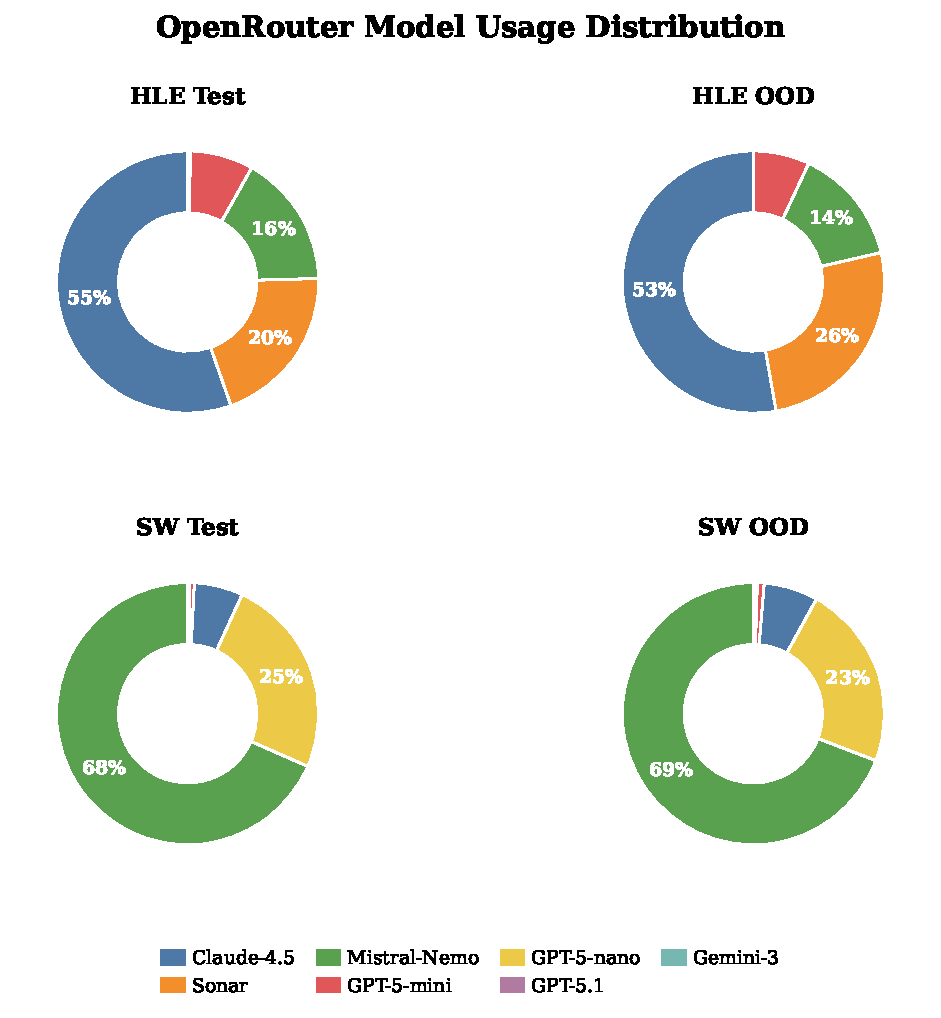
\includegraphics[width=\columnwidth]{figures/openrouter_model_usage.pdf}
\caption{Model usage distribution of OpenRouter on ScienceWorld and HLE. On ScienceWorld, OpenRouter predominantly selects lightweight models (Mistral-Nemo: 68\%, GPT-5-nano: 24\%), while on HLE it primarily uses stronger models (Claude-4.5: 54\%), reflecting different difficulty assessments.}
\label{fig:openrouter_model_usage}
\end{figure}


\section{Prompts and Tool Schemas}
\label{app:prompts}

We report the prompts used in our evaluation setup. For brevity, we omit the format-error correction prompts.

\subsection{ScienceWorld Agent Prompt}
\label{app:prompts:sw}
\input{prompts/scienceworld_system}
\input{prompts/scienceworld_instance}

\subsection{HLE Agent Prompt}
\label{app:prompts:hle}
The HLE system prompt injects tool schemas via a template variable. We list each tool schema explicitly in Appendix~\ref{app:tool_schemas}.
\input{prompts/hle_system}
\input{prompts/hle_instance}

\subsection{Tool Schemas}
\label{app:tool_schemas}
We list each tool's JSON schema (name, description, and parameter schema) used by the HLE agent.
\input{prompts/tool_schema_search_json}
\input{prompts/tool_schema_browse_json}
\input{prompts/tool_schema_python_json}
\input{prompts/tool_schema_answer_json}

\subsection{Routing Model Prompt for LLM Router / Router-R1}
\label{app:prompts:routing}
We report the turn-level routing prompt used by the LLM Router baseline and by Router-R1. In both baselines, the routing model is queried at each turn to produce a \texttt{<select>} decision. They use the same prompt template; Router-R1 uses a trained \texttt{Qwen2.5-7B-Instruct} routing model, while LLM Router directly uses \texttt{DeepSeek-V3.2} (no training).
\input{prompts/llmrouter_system}
\input{prompts/llmrouter_model_descriptors}

\subsection{Browse Extractor Prompt}
\label{app:prompts:browse}
The HLE \texttt{browse} tool can optionally use an LLM to extract and summarize relevant evidence from retrieved webpages. We report the extractor prompt used for this LLM-based summarization.
\input{prompts/browse_extractor_prompt}

\subsection{HLE Judge Prompt}
\label{app:prompts:judge}
HLE scoring uses an LLM-as-a-judge component aligned with the official HLE evaluation. We report the judge prompt used to compare a model response against the provided reference answer.
\input{prompts/hle_judge_prompt}
